A potential source of error in opening angle measurements is the scattering of neutrons within the fission target.
This is a cause for concern because when neutrons scatter from heavy nuclides, such as $^{238}$U, they are likely to be deflected at large angles, resulting in n-n opening angles that do not reflect the true underlying fission kinematics.
The effect that this has on this work is assessed by MCNP simulations.
In summary, for 6\% of n-n pairs, at least one neutron out of the two scatters before exiting the target, according to the simulation.
This effect does not have a large influence on the measured $\theta_{nn}$ distribution according to the data shown in Fig.~\ref{fig:ElasticScatteringEffect}.

The rate of elastic scattering is affected by the size and shape of the target.
A thin strip is the ideal target shape regarding the rate of neutron elastic scattering per unit of total target volume.
See Fig~\ref{fig:ElasticScatteringPlot} for the simulated elastic scattering rates for both thin strip and cylindrical shaped targets.
The simulation indicated that the rate of elastic scattering in cylindrical targets is about a factor of two times greater than in thin strip targets with the same volume.
\begin{figure}
    \centering
    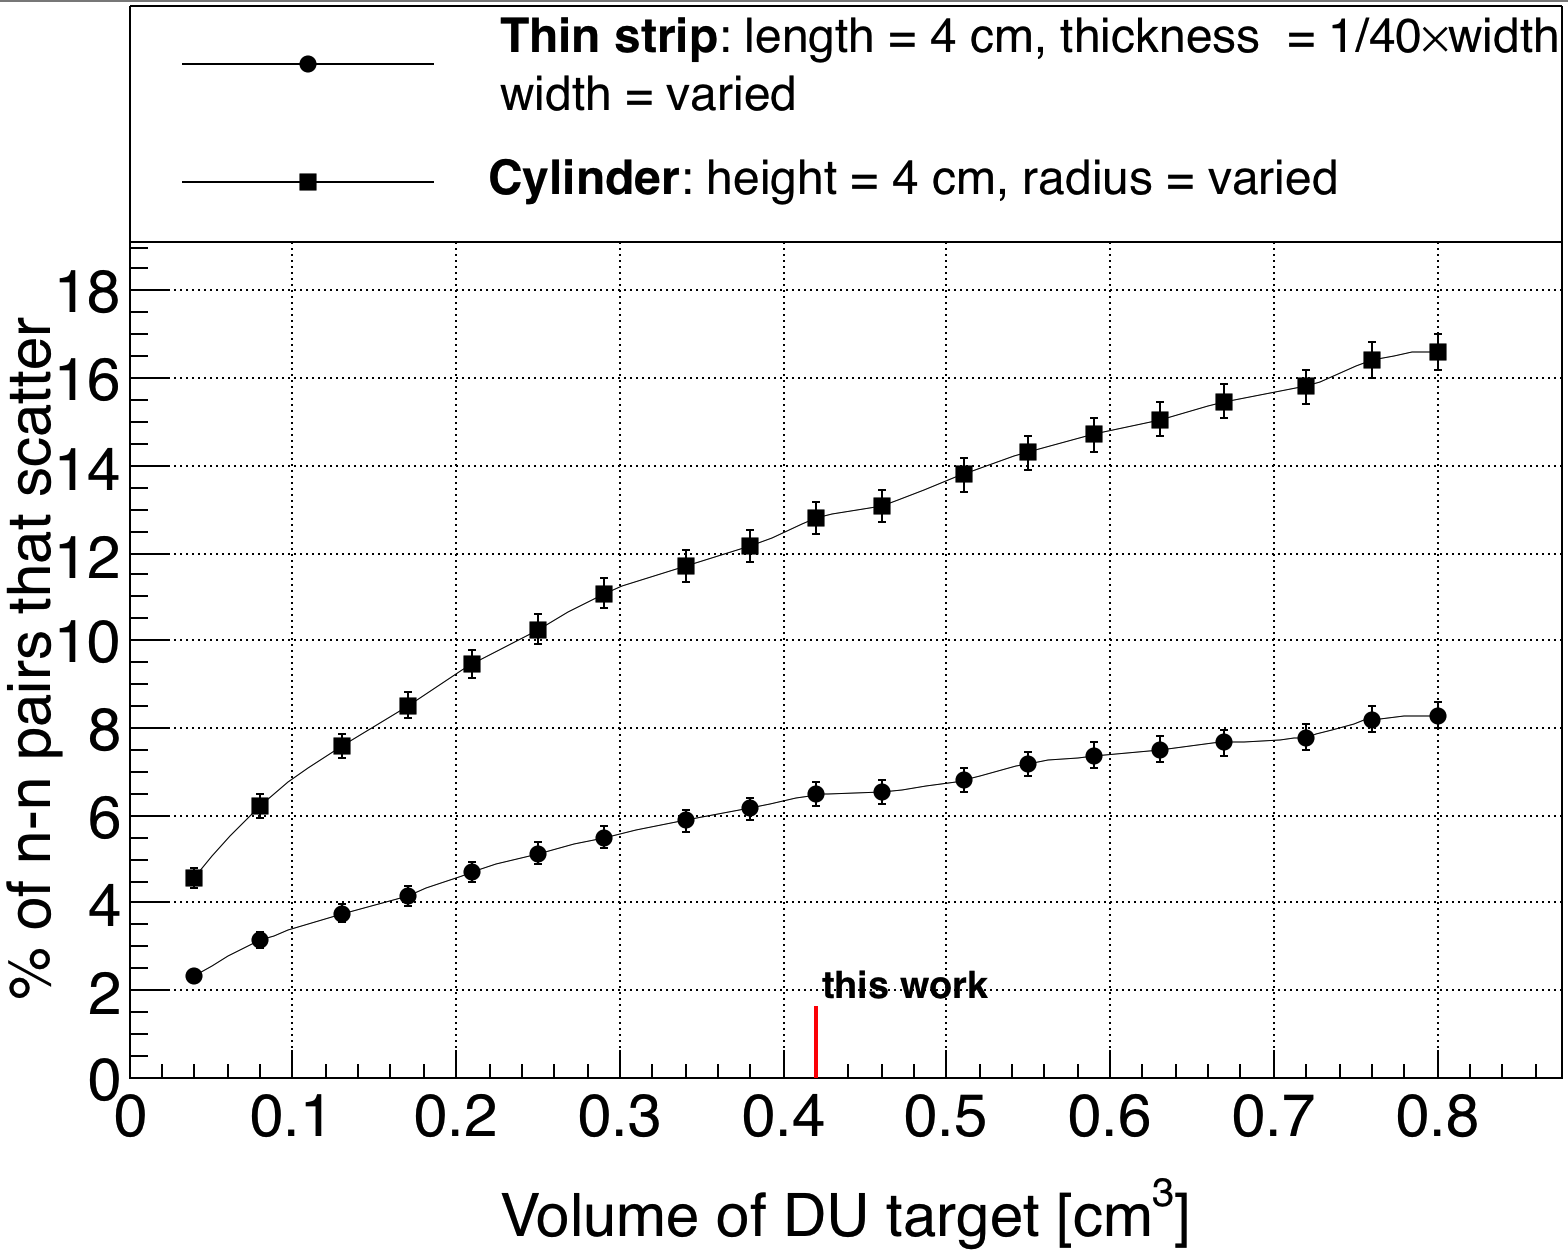
\includegraphics[width = \figsize\textwidth]{ElasticScatteringPlot.png}
    \caption{
     Result of an MCNP simulation in which n-n pairs, with energies sampled from a typical watt fission spectrum, were generated uniformly throughout the volume of DU targets.
        The y-axis is the rate of opening angle contamination due to the scattering of, within the DU target in which they were produced, either one or both of a pair of neutrons.
    The lack of symmetry of a thin strip target can be removed by slowly rotating the target around the vertical axis during data acquisition, making it the optimal target geometry for the minimization of the rate of neutron scattering.
    The target used in this work had a length of 4~cm, a width of 2~cm, and a thickness of 0.05~cm.
    }
    \label{fig:ElasticScatteringPlot}
\end{figure}

The target's dimensions are small enough that the rate of photon absorption, and thus photo-neutron production, is virtually uniform throughout the entire target volume.
An MCNP-PoLiMi simulation was used to generate $^{252}$Cf spontaneous fission events uniformly throughout the target.
The SF of $^{252}$Cf is used instead of the photofission of $^{238}$U because of the current lack of photofission models, however, the underlying fission kinematics are, broadly speaking, the same for the SF of $^{252}$Cf and the photofission of $^{238}$U, thus, the two processes have similar n-n correlations.

Section~\ref{sec:anomaly} discusses the observation of an unexpected drop in correlation around 180$^{\circ}$ in our photofission of $^{238}$U measurement, as seen in Figs.~\ref{fig:DU(0)} and \ref{fig:DU(2)}.
This motivated a second simulation regarding elastic scattering which examined whether this decrease in the correlation around 180$^{\circ}$ opening angles reflects the underlying physics of the fission process.
In particular, note that throughout these measurements, the target was continuously rotated once per 8 seconds.
This means that for the determination of the uncorrelated opening angle distribution, the trajectories of the two neutrons were taken from two different pulses in which the target was at a different orientation for each of them.
Additionally, each of the neutrons likely originated from different regions of the target volume.
On the other hand, for the same-pulse, correlated neutron measurement, the target was in the same orientation and the two neutrons were generated at the same position in the target.
For these reasons, the rates of neutron scattering within the target are not necessarily equal for the same-pulse and different-pulse cases.
As such, we investigated whether these differences could cause this apparent decrease in the opening angle distribution.

Using the correlated $^{252}$Cf SF source built-in to MCNP-PoLiMi, the opening angle distribution of neutrons at the moment of emission, labeled \emph{true} in Fig.~\ref{fig:ElasticScatteringEffect}, were compared to that the neutrons after they have escaped the target, labeled \emph{reconstructed} in Fig.~\ref{fig:ElasticScatteringEffect}.
The location of fission events were sampled uniformly throughout the targets volume.
The analysis employs the same technique outlined in section~\ref{subsec:SPDPCancelation}, in which a correlated neutron distribution is divided by an uncorrelated neutron distribution.
The correlated neutron distribution is formed by pairing neutrons emitted during the same fission, and the uncorrected distribution by the pairing of neutrons emitted during different fissions.
In order to account for the effect of a rotating target on the trajectories of neutrons from different-pulses, the coordinate system was rotated about the vertical axis accordingly for different fission events.
The result from this simulation suggests that the rotating 0.05$\times$2$\times$4~cm$^3$ U-238 target does not, due to neutron scattering, result in a significant departure from the true n-n opening angle distribution.

%Aside from the size, shape, and continuous rotation of the target, the rate of neutron scattering within the target of detected neutrons is also affected by the fact that the detection system does not have 4$\pi$ coverage.
%The target is itself asymmetrical, and thus not all exit trajectories for a photo-neutrons are created equal regarding the scattering probability.
%The detection system's limited geometrical coverage has the potential to favor some neutron trajectories over others, possibly causing a relative tendency to detect scattered n-n pairs for particular opening angles.
%The potential for this to affect the measurement is captured in the simulation by only counting neutrons which enter a physical volume at which a detector was located during the experiment.
%This distribution is labeled \emph{reconstructed} in Fig.~\ref{fig:ElasticScatteringEffect}, and includes the effects of neutron elastic scattering within the target together with the geometric coverage of the neutron detection system.
%Plotted alongside the reconstructed distribution is the opening angle distribution of the neutrons at the moment immediately after emission, labeled \emph{true}.
%A neutron energy cut of 0.4 MeV is applied to all neutrons in both cases in order to be more reflective of the measurement.
%Fig~\ref{fig:ElasticScatteringEffect} compares the n-n opening angle distribution at the moment immediately after emission (denoted by \emph{true} in figure) to that of neutrons once they have escaped the target (denoted by \emph{reconstructed} in figure).
\begin{figure}
    \centering
    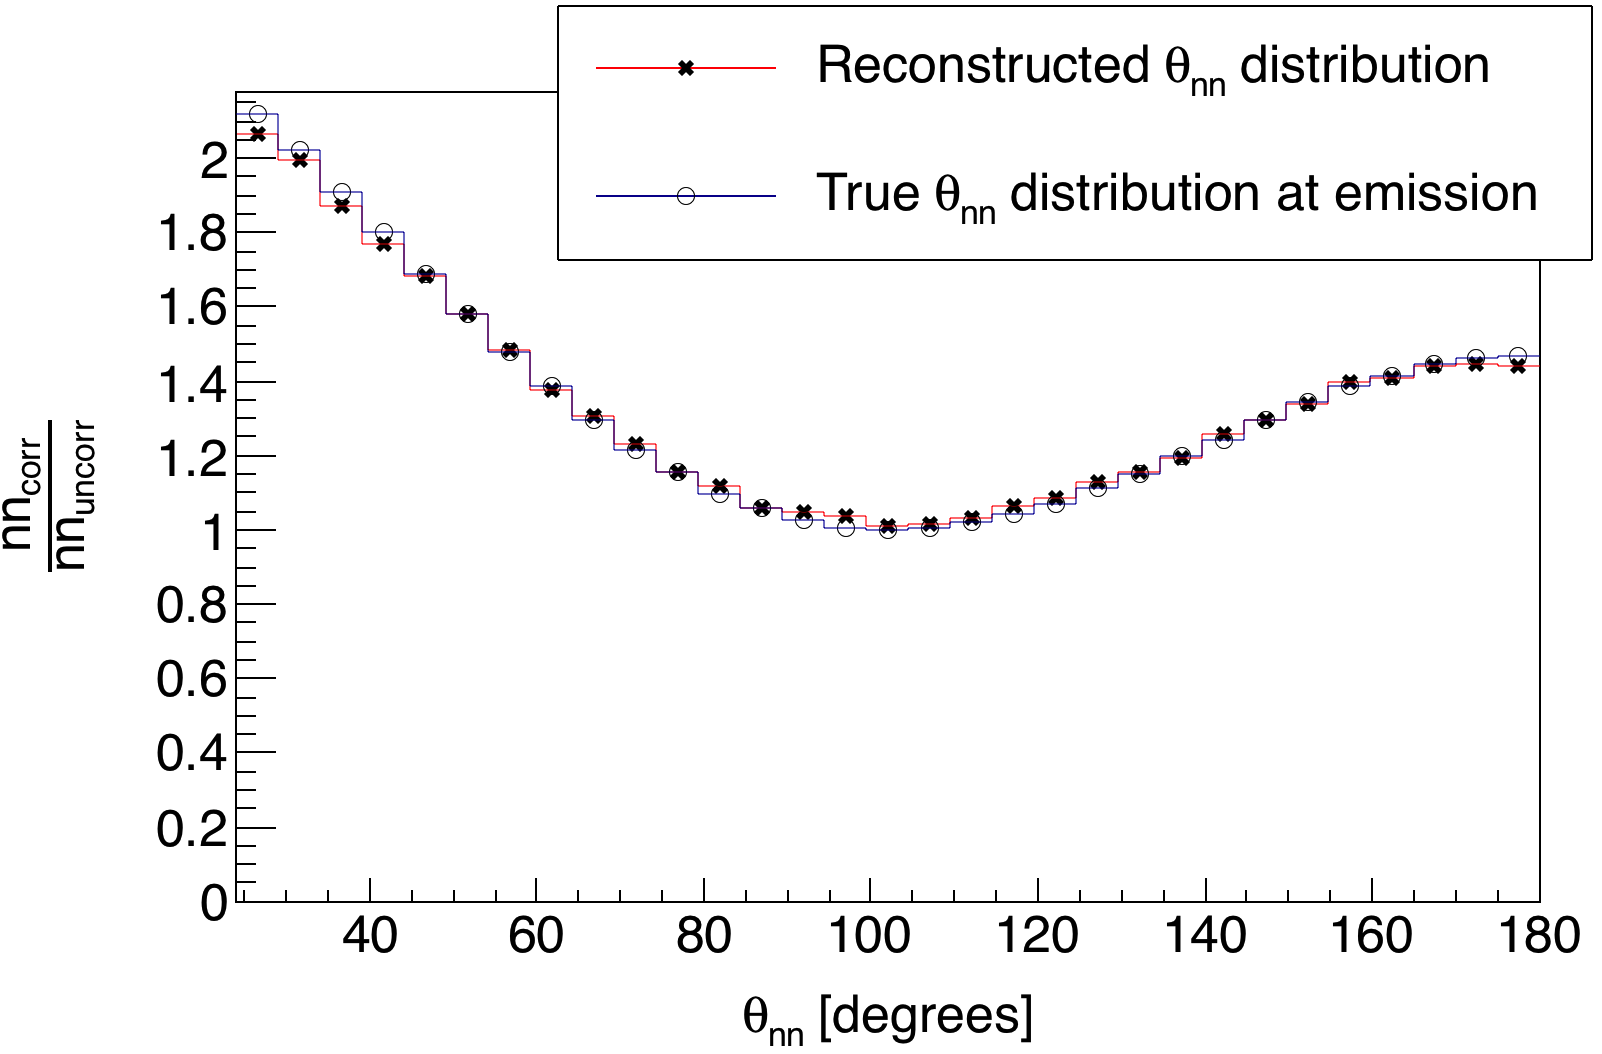
\includegraphics[width = \figsize\textwidth]{EffectOfElasticScattering.png}
    \caption{
    MCNP-PoLiMi simulation of correlated $^{252}$Cf neutrons sampled uniformly throughout a 0.05$\times$2$\times$4~cm$^3$ U-238 target.
    The slight difference between the curves is due solely to the elastic scattering of neutrons within the target, since detector physics was not simulated.
    In the reconstructed $\theta_{nn}$ distribution ({\tiny \ding{54}}), only neutrons which enter a physical volume at which a detector was located during the experiment are counted.
   The true $\theta_{nn}$ distribution at the moment of emission is also plotted ($\mathlarger{\mathlarger{\mathlarger{\circ}}}$).
    }
    \label{fig:ElasticScatteringEffect}
\end{figure}